\section{Out-of-sample validation on independent data}\label{sec:validation}

Every physics component of the architecture, and the sensing pattern
itself, is confronted with an experimental dataset it was never fitted
to: the supplementary data of \citet{scott2024silica}, read with the
parameterization corrections of \citet{scott2024corrigendum}. The
corpus comprises 61 monomeric-silica decay experiments and 1{,}275
points spanning 23--80~$^{\circ}$C, pH 2.1--10.0 and ionic strength
0.01--0.53~mol/kg. Because the source is machine-readable, manual
transcription protocols give way to automated parser integrity checks:
unit-header pinning, monotonicity, separation of replicate runs listed
under duplicated identifiers, and flagging of one colloid-regime
outlier that falls outside the dissolved-monomer scope.

\subsection{Kinetics: what a 1979 law does and does not predict}

Two properties of the fitted core are tested separately, because they
fail differently. Consider first the functional form. Linearizing the
integrated $n$-th-order decay law and sweeping $n \in \{2,\dots,6\}$
per experiment shows that single-curve monomer decay in the modern data
is cleanly second order in supersaturation: median $R^2 = 0.992$ at
$n = 2$, degrading monotonically as the assumed order rises, with
best-fit order 2 in all eleven qualifying near-neutral experiments
(Fig.~\ref{fig:kinval}). This does not contradict the source of the
core. The classical ``fourth order'' is a correlation of maximum rate
against initial supersaturation across separate batches, a peak-rate
law, whereas the integrated decay of a single curve follows
Rimstidt--Barnes-type second-order
kinetics~\citep{rimstidt1980kinetics}. The two describe different
observables, and we report both rather than forcing either onto data
that says otherwise. Now the rate level. The observed second-order
constants follow an Arrhenius trend with $E_a \approx 22$~kJ/mol, and
the effective decay constant implied by the fitted core differs from
observation by a factor of about six at the median. That number does
double duty in this paper. It calibrates the adverse stress of
Section~\ref{sec:stress}, and it is the measured size of the gap the
learned residual exists to absorb: no single transcribed rate law
reproduces independent modern data.

\begin{figure}[t]\centering
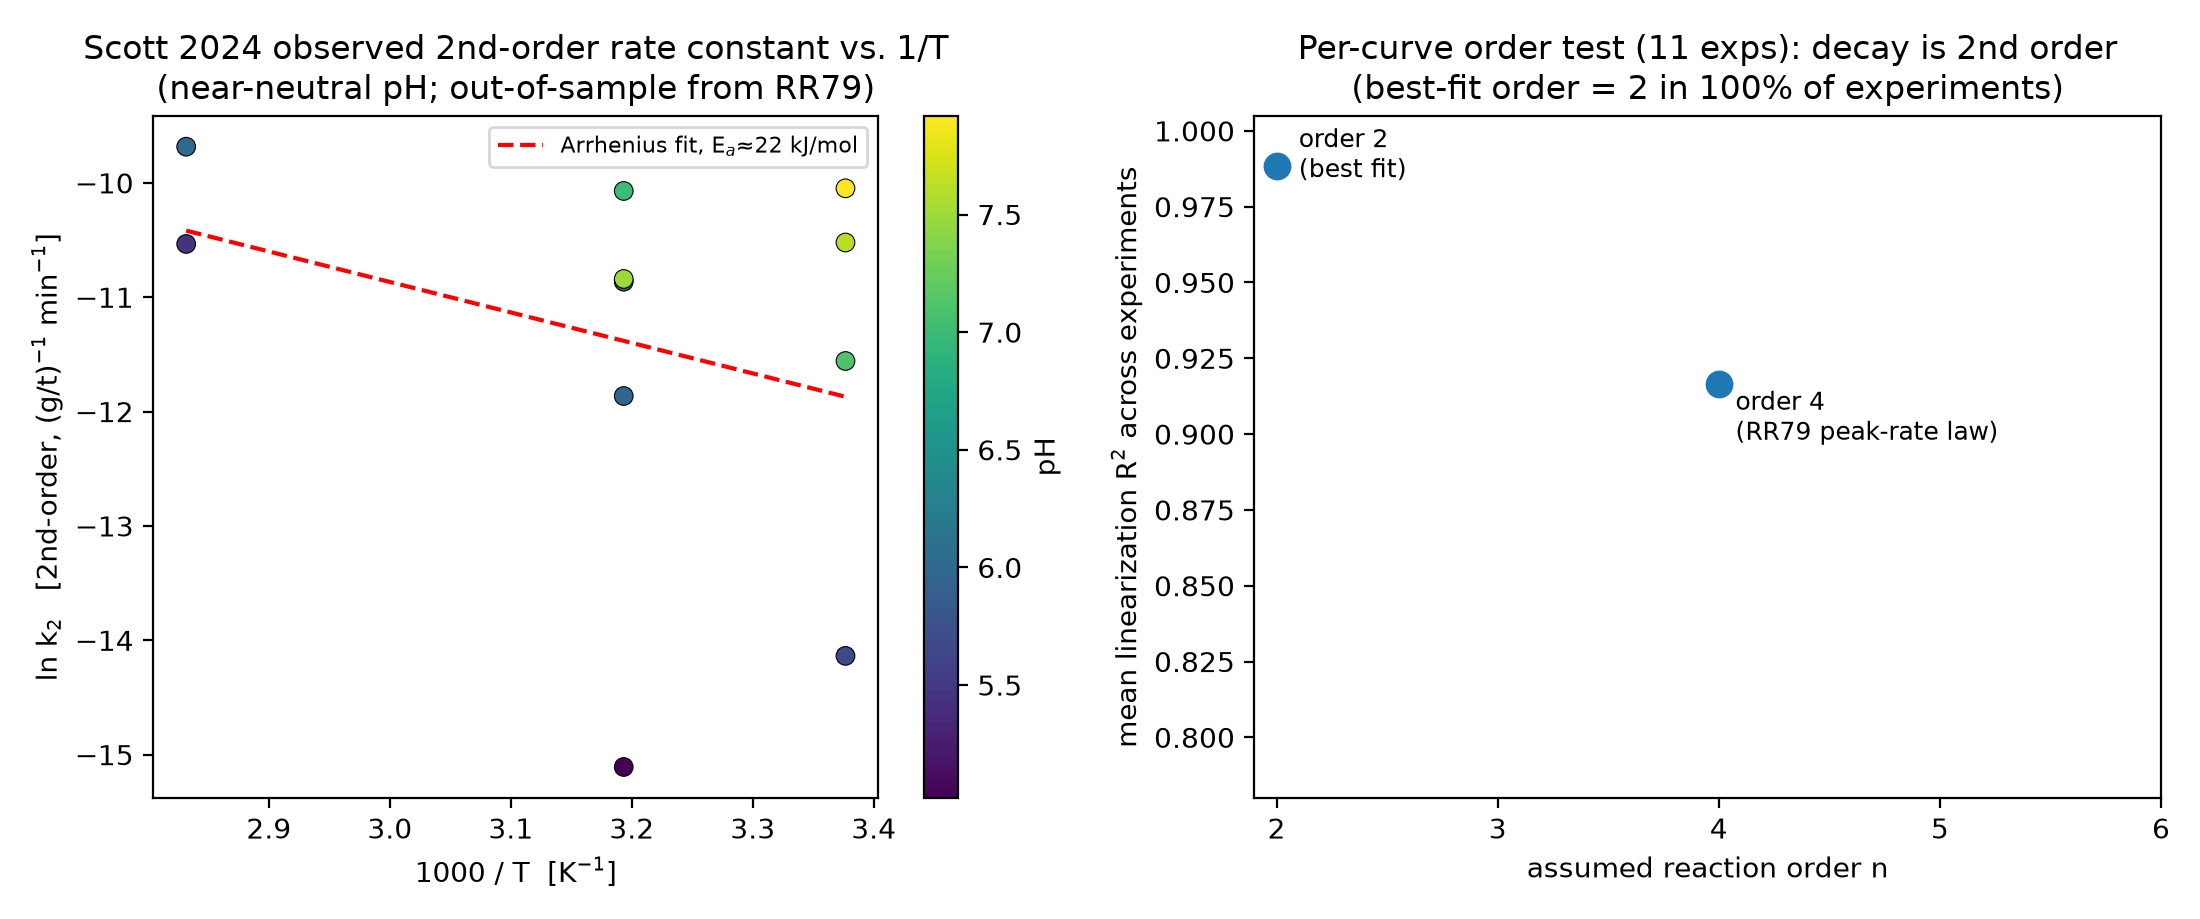
\includegraphics[width=.95\linewidth]{fig_kinetics_validation.png}
\caption{Out-of-sample kinetic validation against
\citet{scott2024silica}. Left: observed second-order rate constants
versus inverse temperature for the near-neutral experiments, with the
Arrhenius trend. Right: mean linearization $R^2$ versus assumed
reaction order; single-curve decay is second order, while the
fourth-order form is a peak-rate law. Source:
\texttt{results/kinetics\_validation.csv}.}
\label{fig:kinval}
\end{figure}

\subsection{Solubility: mutual validation across 24 years}

The plateau of a near-complete decay experiment is an independent
measurement of amorphous-silica solubility. Sixteen near-neutral
experiments that consumed at least 70\% of their initial
supersaturation plateau at 0.90--1.37 times the
\citet{gunnarsson2000amorphous} correlation, with a median of 1.05. The
2000 correlation and the 2024 endpoints therefore validate each other
in both directions, and the measured band $[0.90, 1.37]$ becomes the
solubility axis of the sensitivity study in Section~\ref{sec:sobol}.

\subsection{The sensing pattern on real curves: identifiability
precedes correction}\label{sec:sensorval}

Finally, the field sensing pattern is replayed on laboratory truth.
Each qualifying experiment is treated as a plant, interval-average
observed rates as the hidden truth, the fitted core as the prior, and
only the first $K$ intervals as labels. Three arms with honestly
counted parameters are compared: the core alone; a one-parameter scalar
hybrid, a fitted log-level offset that is deployable from a single
label, where a data-only fit cannot operate at all; and a two-parameter
affine hybrid whose slope in $\ln s$ is, by construction, an order
correction. Second-order truth against a fourth-order core predicts
$b \approx -2$.

The raw affine arm is retained as a cautionary ablation. Early labels
span almost no state (a label $\ln s$ spread of 0.047 against a test
span of 2.61), so unregularized slopes explode, with $b$ ranging from
$-230$ to $+769$, and the arm performs far worse than no correction at
all. Applying the same credibility mechanism as the field sensor, a
leave-one-out selection between the scalar and a clipped affine, the
correction collapses to the safe scalar whenever the labels have not
earned the slope ($K \le 3$). At $K = 5$ it engages in 9 of 21
experiments with median $b = -2.50$, independently re-measuring the
order-2 finding, and wins outright with a median RMSE of 2.59 against
3.04 for the core (Fig.~\ref{fig:sensorval}). The principle this
crystallizes, identifiability precedes correction, also explains the
field results. A plant regulated near an operating point presents a
level-dominated, label-covered correction problem, which is exactly
where hybrid residuals win; wide-range extrapolation demands
state-spanning labels, and a credible architecture must know which
regime it is in.

\begin{figure}[t]\centering
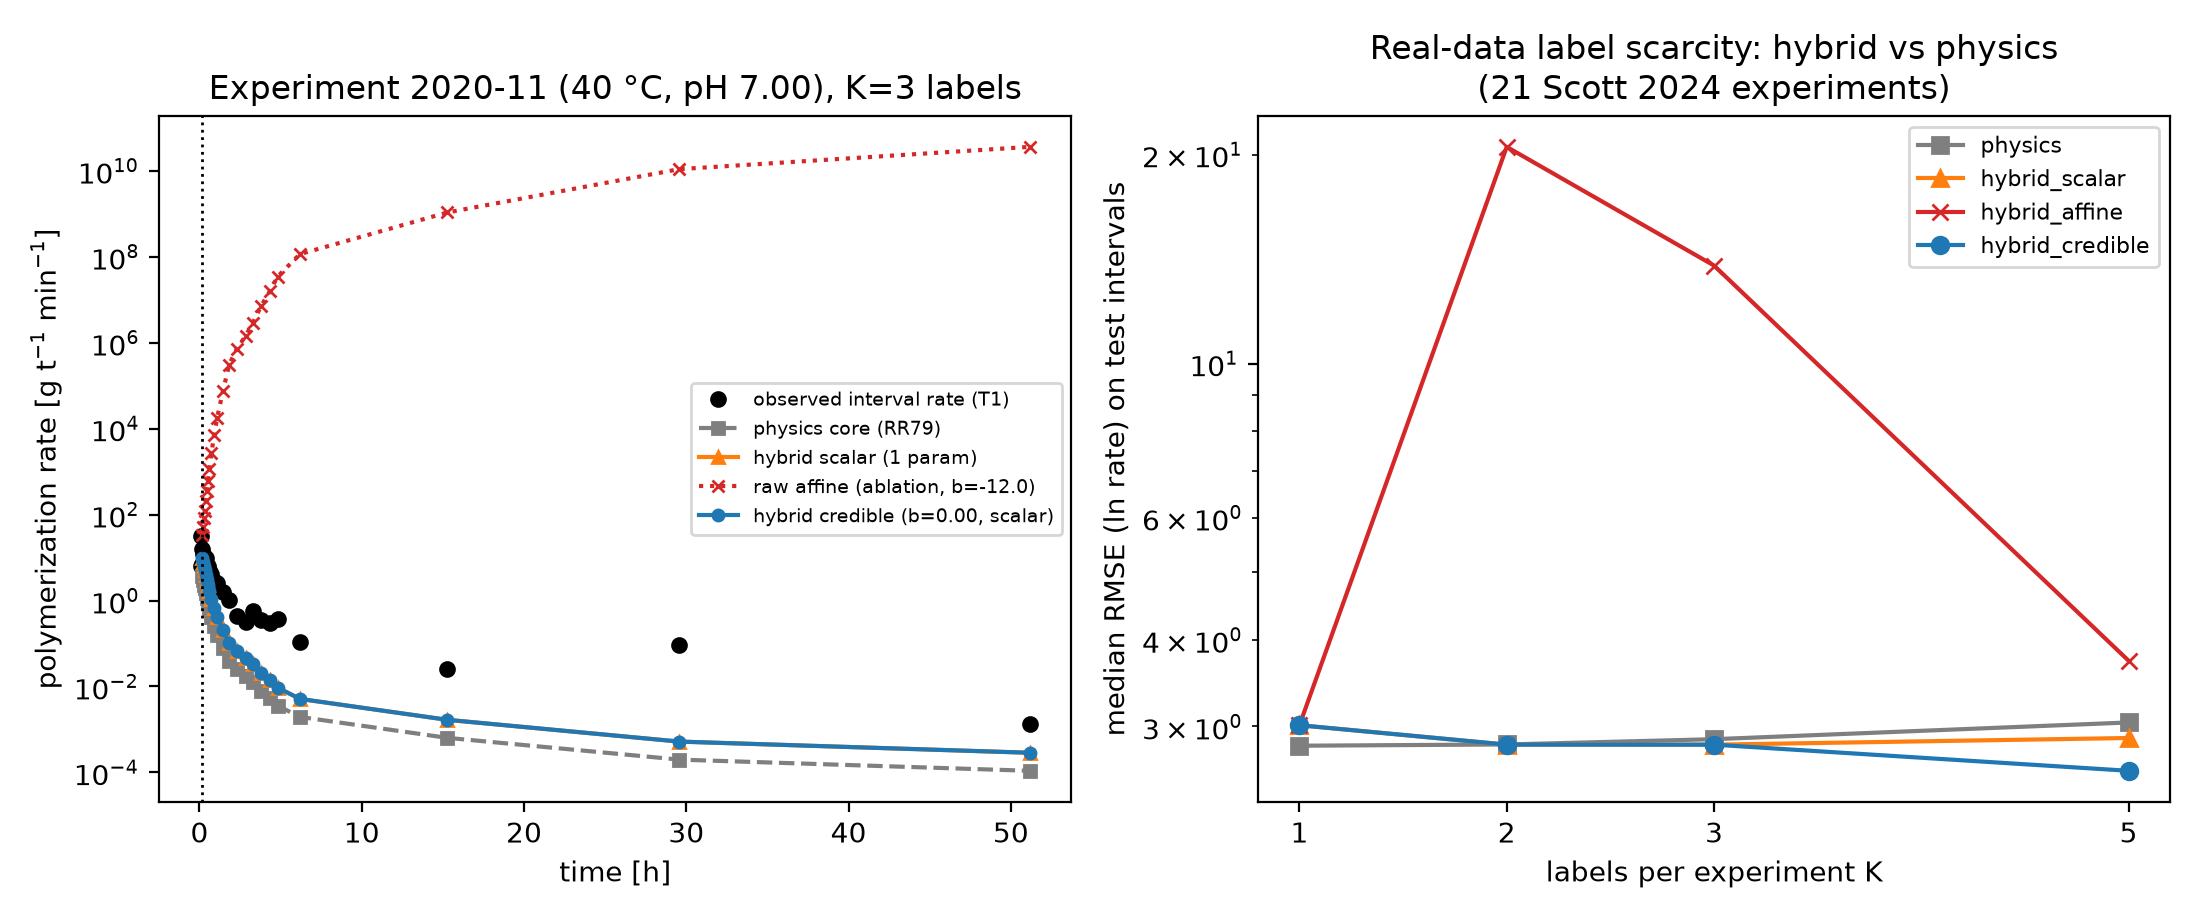
\includegraphics[width=.95\linewidth]{fig_sensor_validation_scott.png}
\caption{The sensing pattern on real decay curves. Left: a
representative experiment, showing the observed interval rates, the
diverging physics core, the raw-affine explosion, and the credible
hybrid. Right: median test RMSE versus labels per experiment $K$ for
all arms, on a log scale. Source:
\texttt{results/sensor\_validation\_scott.csv}.}
\label{fig:sensorval}
\end{figure}
